\maketitle
\vspace*{5mm}
\tableofcontents
\listoffigures
\listoftables

\newpage

\thispagestyle{fancy}

\newcommand\PredstaveniSpolecnosti{PŘEDSTAVENÍ SPOLEČNOSTI Proxy, a.s.}
\begin{lefttextpipe}
	{\huge \PredstaveniSpolecnosti}
\end{lefttextpipe}
\phantomsection
\addcontentsline{toc}{section}{\PredstaveniSpolecnosti}

Předmětem podnikání společnosti je především \textit{daňové poradenství} a \textit{činnost účetních poradců, vedení účetnictví, vedení daňové evidence}. Společnost má okolo 60 zaměstnanců\footnote{V Merku je možné dohledat číslo 50 - 99 zaměstnanců.}\textsuperscript{, }\footfullcite{proxy_merk} a je lokalizována v České republice. Společnost je součástí většího holdingu PROXY Holding a.s.. Společnost je dělená na několik oddělení, z nichž každá se soustředí na specifickou oblast v rámci daňového a účetního poradentsví, každá z těchto oblastní má vlastního manažera. Obecné směřování společnosti je stanovováno představenstvem.\\

Společnost se pohybuje výhradně na českém trhu v oblastni daňové a účetní, jejímy klienty jsou subjekty, které v České republice vykonávají jakoukoli ekonomickou činnost v rámci které jsou povinny řídit se českými daňovými a účetnímy předpisy. Hlavní službou společnost Proxy, a.s. je tak poskytování služeb související právě s činnostmi týkající se daní a vedení účetnictví a jedná se tedy výhradně o účetní a daňovou společnost.

\section*{A. Současná vize a poslání podniku}
\label{sec:Vize a poslani}
\addcontentsline{toc}{subsection}{\nameref{sec:Vize a poslani}}

\subsection*{A.1 Poslání a mise společnosti}
\label{sec:Poslani}
\addcontentsline{toc}{subsubsection}{\nameref{sec:Poslani}}

Dle informací na webových stránkách společnosti je základní poslání a mise poskytování služeb na poli daňového poradenství, účetnictví, mzdové evidence a dalšího specializovaného poradenství\footfullcite{proxy_website}, především pro zahraniční investory vstupující na český trh a zjednodušit a zpřehlednit jim tam investici a fungování v České republice. 

\subsection*{A.2 Vize}
\label{sec:Vize}
\addcontentsline{toc}{subsubsection}{\nameref{sec:Vize}}

Vize společnosti spočívá především v tom, aby se stala partnerem pro své klienty a nadále je podporovala kvalifikovaným poradenstvím a to jak pro českou, tak i pro mezinárodní klientelu. Společnost se stala v roce 2004 součástí mezinárodní asociace poradenských firem HLB se sídlem v Londýně a nadále tak podporuje svojí vizi o kvalitní poradenské činnosti v dané oblasti\footfullcite{proxy_o_firme}.

\subsection*{A.3 Aktuální problémy}
\label{sec:Problemy}
\addcontentsline{toc}{subsubsection}{\nameref{sec:Problemy}}

%Problémy jsou příležitosti.

%Problém bude škláování a legislativní požadavky a jejich implementace a přenesení do procesů týkající se poradenství v oblasti daní a činnosti daňových poradců a účetních poradců a udržování knowledgebasu.

%Dále školení lidí, tato oblast je dost problematická, rovněž taky shánění lidí?

S ohledem na informace na webové stránce společnosti a finanční výkazy (viz analýza v části \textit{D. Současné cíle společnosti}) se společnost nepotýká s nedostatkem příležitostí a z nichž pramenícího zisku. Společnost je rentabilní a poptávka po jejích službách, vzhledem k výsledkům této analýzy, je vysoká.\\

Dle informací z Merku a Justice se společnost rovněž nepotýká s žádným právním problémem a není insolventní\footfullcite{proxy_merk}.\\

%\newpage

I s ohledem na výše uvedené informace je však možné vysledovat a odhadnout širší škálu problémů, se kterými se společnost této velikosti a významu potýká a ze své podstaty potýkat musí.\\

Nejzásadnější problémy lze rozdělit do několika kategorií:\\

\begin{itemize}
	\item reakce na poptávku a z toho vyplývající škálování,
	\item reakce na vnější faktory, především na měnící se legislativu,
	\item udržování knowledge base,
	\item rostoucí náklady a mzdy,
	\item roustoucí požadavky kvalifikační požadavky na zaměstnance.
\end{itemize}

\vspace*{5mm}

\newpage

\textbf{Reakce na poptávku, škálování}\\

Jako každá společnost musí i \textit{Proxy a.s.} reagovat na poptávku, pokud chce udržet svojí rentabilitu. Vzhledem k výsledku hospodaření za účetní období (viz graf níže) a vývoj počtu živnostenských oprávnění (viz reakce na konkurenci) lze dovodit, že poptávka po účetních službách dlouhodobě stoupá.

\begin{figure}[!htbp]
	\inputfile{Parts/IntroductionResources/CHART_Vyvoj_zisku}
	\caption[Výsledek hospodaření za účetní rok]{Výsledek hospodaření za účetní rok\protect{\footfullcite{proxy_merk}}}
	\label{fig:vhzur}
\end{figure}

Vzhledem ke zmíněnému růstu výsledků za sledovaná období lze dovodit, že Proxy na tento problém reaguje adekvátně a dokáže ho přeměnit na příležitost.\\

Důležité je však dodat, že nemáme informace týkající se výsledku hospodaření za rok 2020 a za rok 2021\footnote{Autoři jsou si vědomi, že ke dni vzniku této práce nenastala pro subjekt zákoná povinnost uveřejnit účetní závěrku ve sbírce listin.}, neboť listyny dosud nebyly vloženy do sbírky listin\footfullcite{proxy_justice}. Z tohoto důvodu není možné se stoprocentní jistodou dovodit stejné závěry i pro rok 2020 a 2021, z historického vývoje není rovněž možné vycházet vzhledem k probíhající pandemii i jí podnícené změny na trhu. Vzhledem k výsledkům hospodaření za roky předcházející a stále rostoucímu počtu živnostenských oprávnění v daném oboru se autoři domnívají, že lze důvodně dovodit, že trend růstu výsledku hospodaření a tedy přímý výsledek využitých příležitostí by měl mít i pro rok 2020 a 2021 rostoucí charakter. Minimálně za období 2014 až 2019 lze vyhodnotit, že reakce na poptávku ze strany společnosti je více než adekvátní, a že společnosti se podařilo dosáhnout a udržet dlouhodobý růst.\\

%Nemáme však info za rok 2020 a 2021 vzhledem k výsledku hospodaření, ale vzhledem ke stále rostoucímu počtu podnikatelů v dané oblastni (živnostenských oprávnění) lze důvodně dovodit, že poptávka neklesá. Minimálně za období 2014 - 2019 lze vyhodnotit, že reakce na poptávku ze strany společnosti je více než adekvátní a že společnosti se podařilo udržet dlouhodobý růst.\\

%\newpage

\textbf{Reakce na konkurenci}\\

Jako káždá společnost je potřeba reagovat na konkurenci.

\begin{figure}
	\inputfile{Parts/IntroductionResources/CHART_Ziv_number_in_time}
	\caption{Počet živností}
	\label{fig:pz}
\end{figure}

\textbf{Reakce na měnící se legislativu}\\

\textbf{Udržování knowledge baseu}\\


škálování vzhledem k dlouhodobému ekonomickému růstu a větší poptávce po daňovém a účetním poradenství, toto lze dovodit s ohledem jejich stránku kde chtějí studenty a mají permanentně vyvěšené pracovní nabídky, ČSÚ a vývoj počtu podnikatelů v dané oblastni a růstu vykazovanému v účetniství. Lze soudit ze statistik MPO odkaz za sledované období čtvrtého, respektive třetího kvartálu od roku 2016 až 2021

Ahoj.
Data2 2

Hello?
%\inputfile{Parts/IntroductionResources/CHART_Vyvoj_zisku}

%\begin{center}
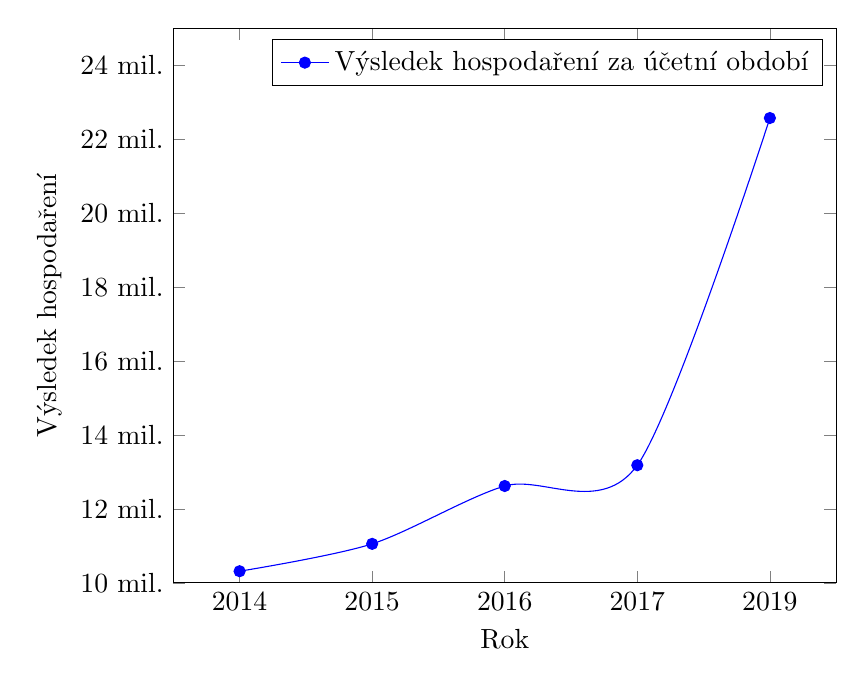
\begin{tikzpicture}
	\begin{axis}[
		width=10cm,
    	xlabel=Rok,
    	ylabel=Výsledek hospodaření,
    	xmin=0, xmax=100,
    	ymin=10, ymax=25,
    	xtick={10,30,50,70,90},
    	xticklabels={2014,2015,2016,2017,2019},   % <---
    	ytick={10,12,...,24},
    	yticklabels={10 mil., 12 mil., 14 mil., 16 mil., 18 mil., 20 mil., 22 mil., 24 mil.}
            ]
		\addplot[smooth,mark=*,blue] 
			plot coordinates {
    			(10,10.314)
    			(30,11.054)
    			(50,12.619)
    			(70,13.181)
    			(90,22.571)
			};
		\addlegendentry{Výsledek hospodaření za účetní období}

	\end{axis}
\end{tikzpicture}
\end{center}

%\input{Parts/IntroductionResources/Diagram}

Taky bych sem měl zařadit analýzu, respektive graf rostoucích příjmů - pak rovněž odkázat na část, kde řeším příjmy v analýze.

Lze možná dooknce usoudit, že nárůst je způsobený i růstem příležitostí během COVIDU 19 a sním spojené nutnosti postarat se o daně a účetnivtví.


 a udržování knowledge basu a přizpůsobování procesů neustále se měnícím požadavkům na daňové a účetní, respektive finanční poradenství a povinnosti s ním související v českém právním prostoru, jedná se tedy o zásadní externí faktor.

\subsection*{A.4 Green deal}
\label{sec:Green deal}
\addcontentsline{toc}{subsubsection}{\nameref{sec:Green deal}}

Společnost Proxy a.s., se ve svých veřejně publikovaných dokumentech společenské odpovědnosti jí vyplývající z jejího postavení vzhledem k životnímu prostředí, a nejenom jemu, nevěnuje.\\

Carbon footprint - office, auta etc.

Společnost se problémem však aktivně nazabývá, což je škoda. Autoři tedy kladou v závěru v projektové části doporučení týkající se zavedení procesů směřující k větší společenské odpovědnosti ve vztahu k udržení přírody a redukce tvorby emisí a dalších pro přírodu negativních dopadů spojených s provozem činnosti subjektu.

Green deal je, odkaz, vztah společnosti ke green dealu je, blabla odkaz. Moc nemusí řešit green deal, nejsou výrobní společnost, která by generovala velké množství znečištění.

\section*{B. Identifikace procesu strategického řízení}
\label{sec:Identifikace procesu strategickeho rizeni}
\addcontentsline{toc}{subsection}{\nameref{sec:Identifikace procesu strategickeho rizeni}}

Úplně nemají, jenom základy podle kterých se řídí a jsou aktualizovány vedením společnosti, jsou v relativně stabilním businessu a pokrývají všechny oblasti v dané kategorii v četně auditu, takže úplně nepotřebují strategický plán.

Majá spíš operativní - na koho, kdy a jak se zaměří - maj i svojí klientelu, takže nepotřebují akvizici tak zásadně.

\section*{C. Popis současného obchodního modelu}
\label{sec:Popis soucasneho obchodniho modelu}
\addcontentsline{toc}{subsection}{\nameref{sec:Popis soucasneho obchodniho modelu}}

Současný model se soustředí na poskytování služeb v oblasti daňové a účetní a auditorské (v rámci jiné společnosti).

\newpage

%\begin{figure}
\inputfile{Parts/IntroductionResources/TABLE_Strategicke_ukazatele}
%	\caption{Test}
%	\label{tab:T}
%\end{figure}

\section*{D. Současné cíle společnosti}
\label{sec:Soucasne cile spolecnosti}
\addcontentsline{toc}{subsection}{\nameref{sec:Soucasne cile spolecnosti}}

\subsection*{D.1 Strategické}
\label{sec:Strategicke}
\addcontentsline{toc}{subsubsection}{\nameref{sec:Strategicke}}

Asi ovládnout trh.

\subsection*{D.2 Taktické}
\label{sec:Takticke}
\addcontentsline{toc}{subsubsection}{\nameref{sec:Takticke}}

Asi takticky ovládnout trh.

\section*{E. Odhad diskontních faktorů}
\label{sec:Odhad diskontnich faktoru}
\addcontentsline{toc}{subsection}{\nameref{sec:Odhad diskontnich faktoru}}

Haha test.

Test \footfullcite{noauthor_fideicommissum_nodate}

$EVA_t = NOPAT_t - WACC_t$ (aktiva celkem$_t -$ krátkodobé závazky$_t$)

%\begin{figure}
\inputfile{Parts/IntroductionResources/TABLE_Konkurencni_vyhoda}
%	\caption{Test}
%	\label{tab:t}
%\end{figure}